\documentclass[a4j]{jarticle}
%\documentclass{jarticle}
\usepackage{conf_jst}
\usepackage{graphicx}
\usepackage{multirow}
\usepackage{listings}
\usepackage{plistings}
%\usepackage{fancyheadings}
\usepackage{longtable}
\usepackage{booktabs}

\oddsidemargin -10mm % 15mm - 1inch(25.4mm)
\evensidemargin -10mm
\textwidth 180mm  % A4幅210mm - 15*2mm
%\topmargin -10.4mm % 25mm - 25.4
\topmargin -10mm % 25mm - 25.4
\textheight 257mm % A4高さ297mm - 25*2mm
%\headheight 10mm
%\headsep 10mm

\setcounter{figure}{0}              %ここで図番号の変更が行えます.
\setcounter{table}{0}               %ここで表番号の変更が行えます.
\setcounter{equation}{0}            %ここで式番号の変更が行えます.

\if0
\def\thefigure{\thesection\arabic{figure}}      %図番号の形式設定
\def\thetable{\thesection\arabic{table}}        %表番号の形式設定
\def\theequation{\thesection\arabic{equation}}  %数式番号の形式設定
\fi

% \tightlistの定義
% これがないとlistがbuild出来ない
\def\tightlist{\itemsep1pt\parskip0pt\parsep0pt}

\setkeys{Gin}{width=7.0cm}  % 図のデフォルトサイズ

\pagestyle{plain}

% \longtableをtwocolumn環境で使えるようにする
\makeatletter
\let\oldlt\longtable
\let\endoldlt\endlongtable
\def\longtable{\@ifnextchar[\longtable@i \longtable@ii}
\def\longtable@i[#1]{\begin{figure}[htbp]
\onecolumn
\begin{minipage}{0.5\textwidth}
\oldlt[#1]
}
\def\longtable@ii{\begin{figure}[htbp]
\onecolumn
\begin{minipage}{0.5\textwidth}
\oldlt
}
\def\endlongtable{\endoldlt
\end{minipage}
\twocolumn
\end{figure}}
\makeatother

\title{20190510\_研究報告資料}
\author{氏名:田村 玄}
\date{期間:2019/11/15 ~ 2020/03/22}

\begin{document}
\maketitle

\section{この期間の研究内容}

\begin{itemize}
\tightlist
\item
  PCの環境設定
\item
  研究グループの選択
\item
  100リンクヘビ型ロボットの確認・修理計画
\end{itemize}

\section{研究の経過と結果}

\subsection{PCの環境設定}

PCにOSをインストールし,ネットワーク,メールエイリアス,プリンターの設定を行った.
そしてNASLINK内に自分用の個人フォルダを作成した.
Office365,ウィルスバスタークラウドなどの基本的なソフトウェアをインストールしたあと,研究に必要なソフトウェアとしてTeX
WorksとVMware Workstatioをインストールした. VMware
Workstatioには,Ubuntu 14.04をインストールした.

\subsection{研究グループの選択}

以前から,ヘビ型ロボットに代表される生物工学というアプローチが,システム工学における重要な要素を多く含んでいると感じていた.
先生や先輩方からヘビグループの研究に関する説明を聞き,ヘビ型ロボットに関する論文を読んだことで,この感覚はさらに大きくなった.
ヘビ型ロボットの研究を経験すれば,「私はシステム工学出身だ」と胸を張って言えそうだと考え,研究グループをヘビグループに決めた.

\subsection{100リンクヘビ型ロボットの確認・修理計画}

100リンクヘビ型ロボットの修理を行う必要があるため,このロボットについて王さんから説明をいただいた.
100リンクヘビ型ロボットの外観をFig.1に示す.
まず,配線がどのようになっているかの説明を受け,コントローラとプログラムの開発環境についての説明を受けた.
コントローラの外観をFig.2に示す.
マイコンボードにはArduinoが使われており,プログラムはC言語で記述する.
またこのロボットの現状の問題点の説明を受け,52リンク以上つなげると正常に動作しないということを聞き,修理手順に関する助言をいただいた.

\begin{figure}
\centering
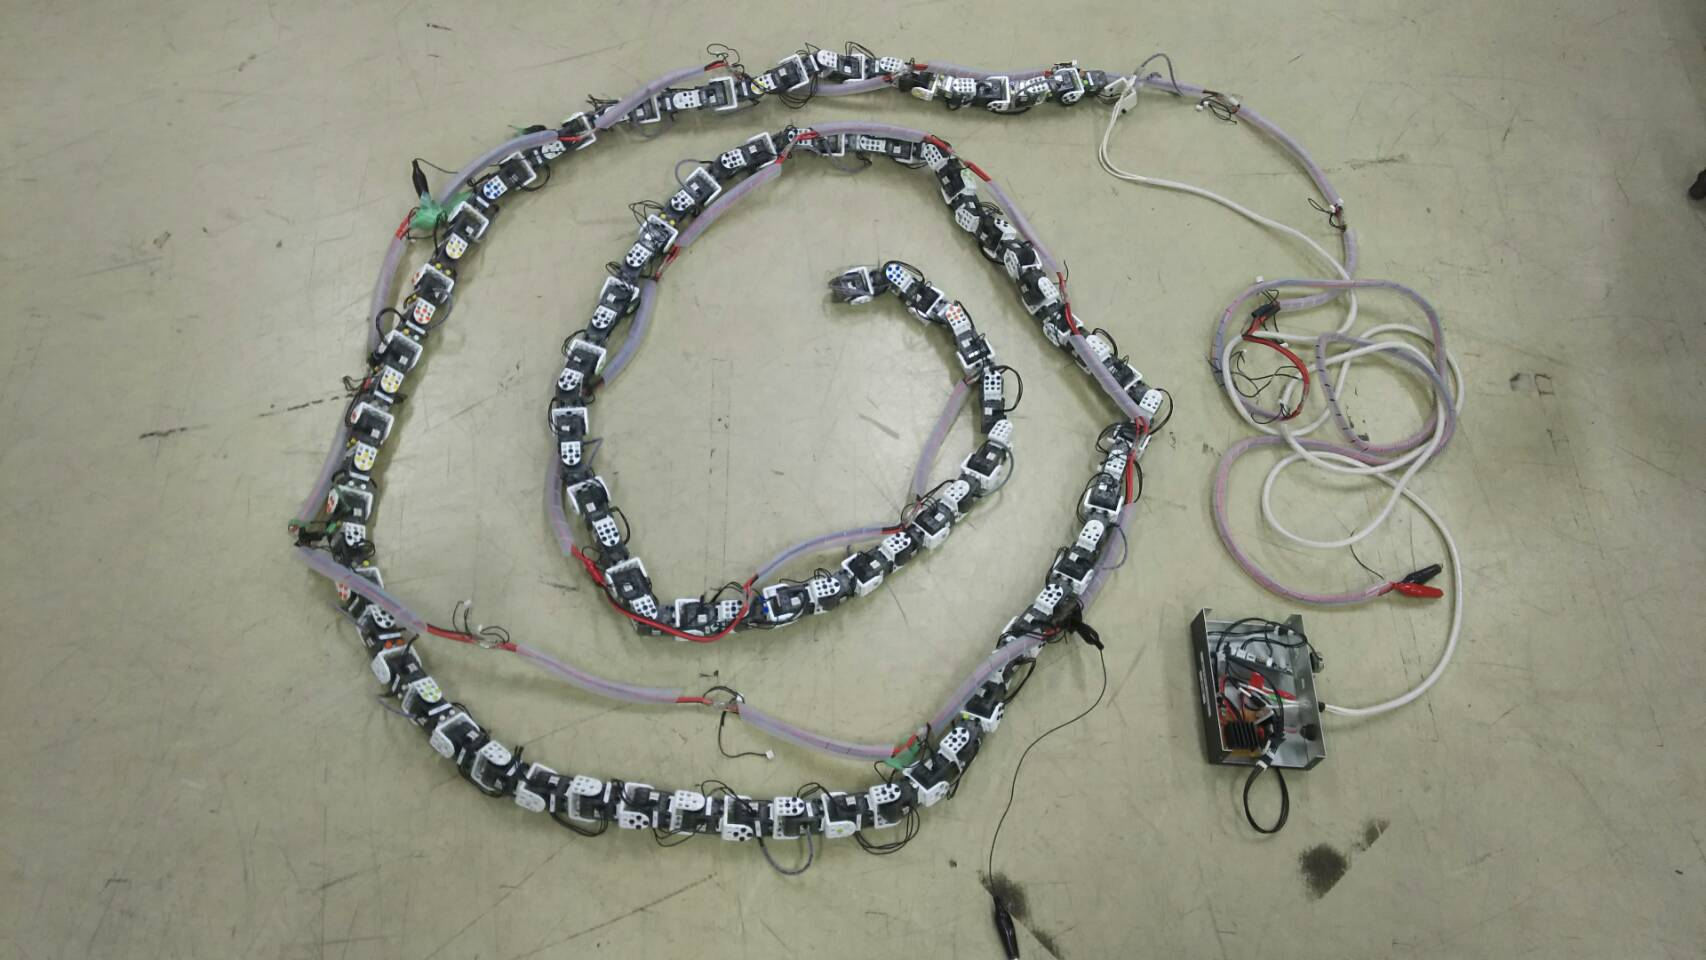
\includegraphics{100リンクヘビ.eps}
\caption{100リンクヘビ型ロボットの外観}
\end{figure}

\begin{figure}
\centering
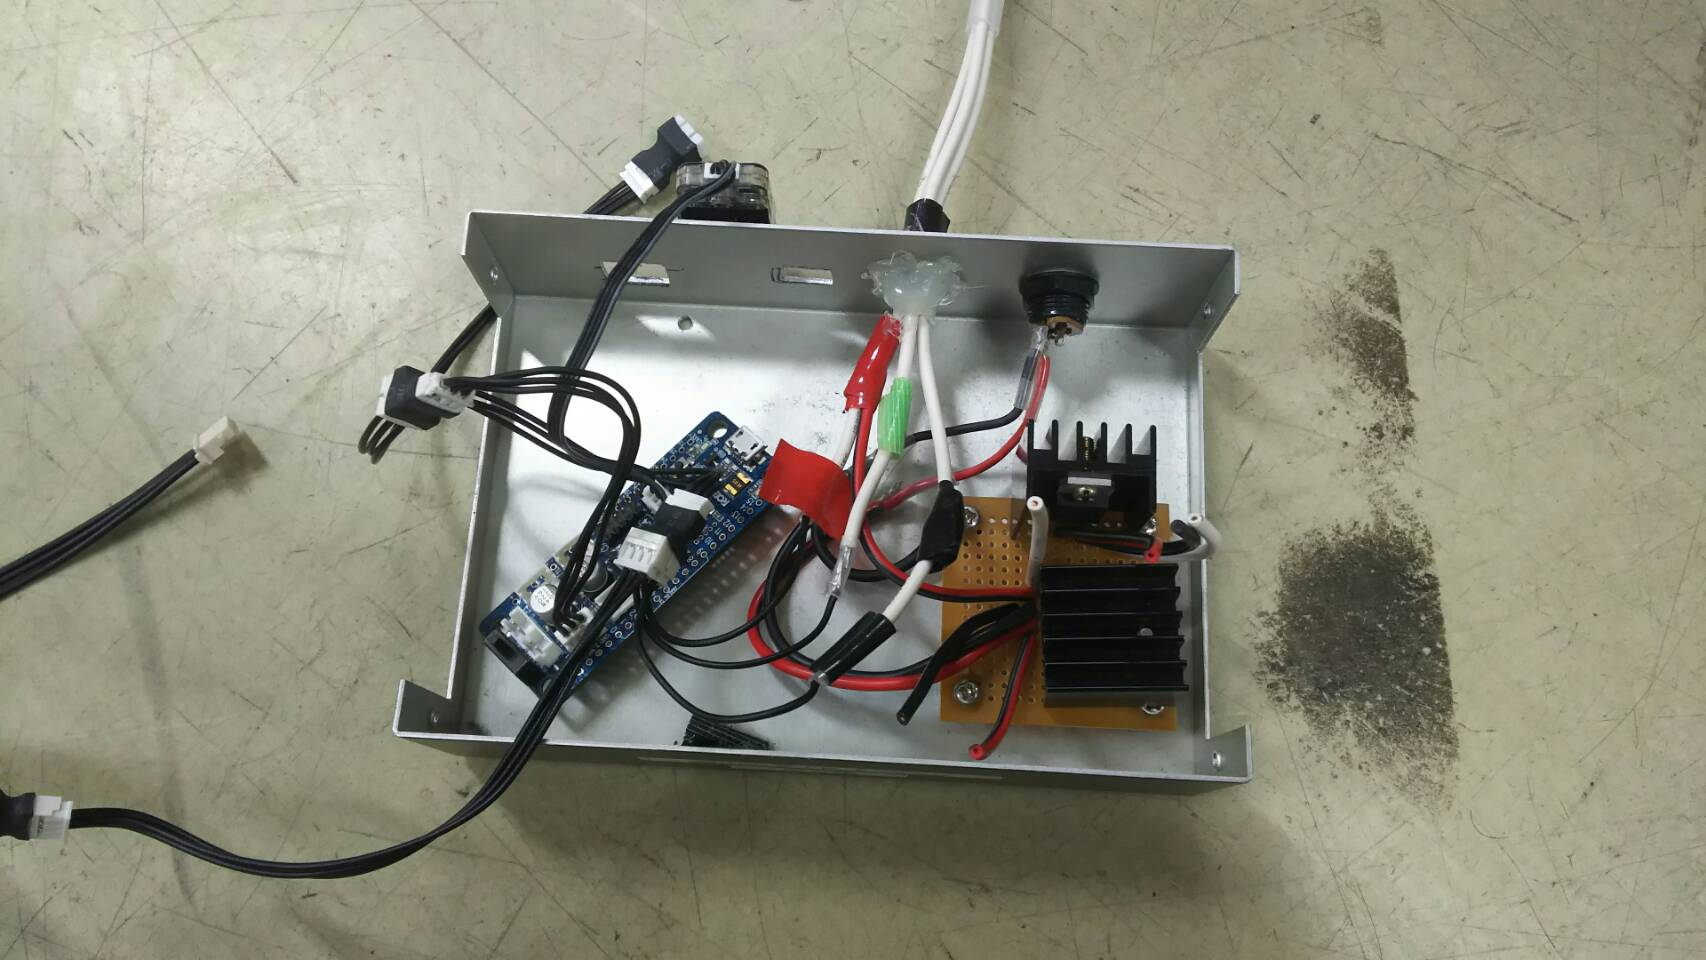
\includegraphics{100リンクヘビコントローラ.eps}
\caption{100リンクヘビ型ロボットのコントローラ}
\end{figure}

その後,もう一人のヘビグループ4回生である久戸瀬と修理計画を立てた.
今回立てた修理計画をFig.3に示す.
勉強もかねて10リンク,50リンクと徐々にリンクを増やして動かしていき,6月13日までに100リンクつなげて動かすことを目標とする.
最大の課題は52リンク以上つなげると正常に動作しないことがであり,これの解決に時間を割けるように計画を立てた.

\begin{figure}
\centering
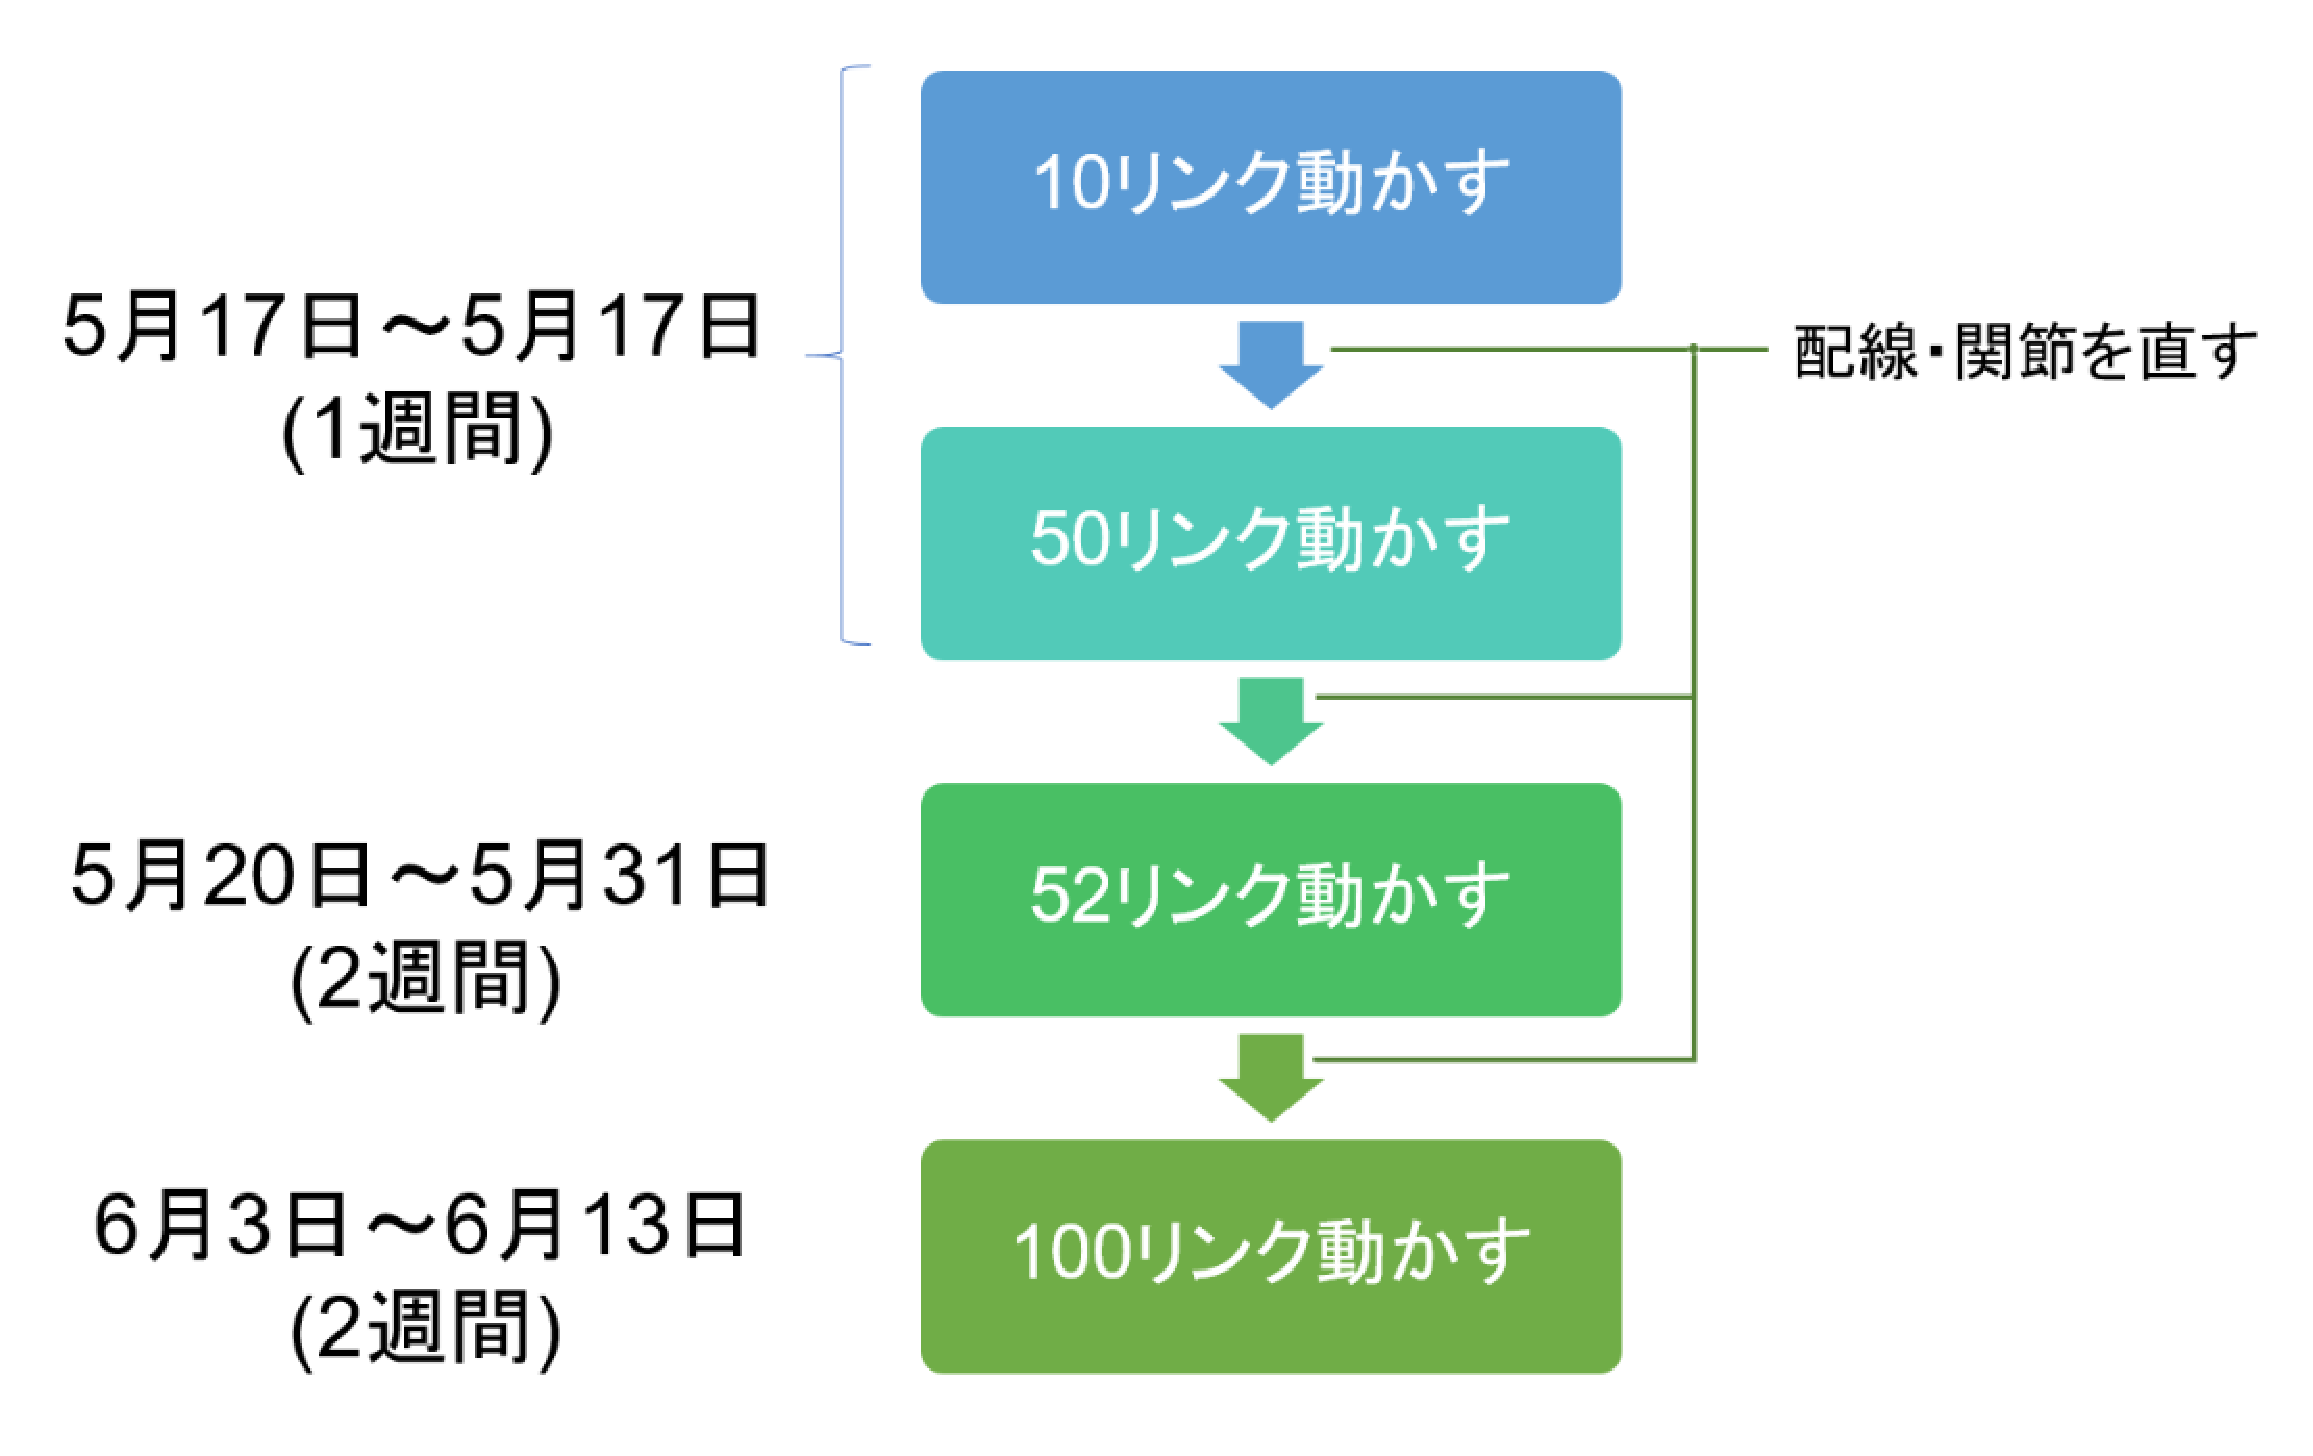
\includegraphics{100リンクヘビ修理計画.eps}
\caption{100リンクヘビ型ロボット修理計画}
\end{figure}

\section{次の期間の研究}

\begin{itemize}
\tightlist
\item
  100リンクヘビ型ロボットを50リンクまで動かす
\item
  ROSのインストール
\item
  広瀬先生の本(生物機械工学)を読む
\end{itemize}

\end{document}
